\chapter{Experiments}\label{chap:experiments}
During this thesis, several experiments were performed in order to evaluate the performance of the framework.
We did different tests of all the parts of the modules, both in simulation and in the real world, in order to understand the weakness of each module and achieve better results.

In this chapter we describe the hardware used in the real world experiments and the software use for the simulations.
Finally, we report the main results achieved during these experiments.
%The system developed, utilize the Robot Operating System (ROS) [19]

\section{Real world hardware}
In all the real world experiments we use only onboard sensing and computing.
An OptiTrack motion-capture system \cite{optitrack} is used to have a ground truth values during some experiments, but the quadrotor never uses these data to fly.

\subsection{Quadrotor}
We utilize custom-designed quadrotors that are based on 3D printed and electronic parts designed in the RPG lab, combined with some commercial components (see Fig.~\ref{fig:quad_hardware}).

These platforms are lightweight (around \SI{500}{\gram}) and safe for operation in proximity with humans. However, they are also agile while maintaining maneuverability and robust vision-based control: they can achieve a maximum speed of at least \SI{4}{\meter \per \second} during vision-based flight.
The quadrotor used is equipped with:
\begin{itemize}
\item an IMU that provides linear accelerations and angular rates;
\item a quad-core single board computer (Odroid XU4), where all computations described in the previous chapters are performed;
\item two different cameras:
\begin{itemize}
\item a downward looking camera with a FoV of \SI{90}{\degree}, used to detect and track the moving platform;
\item a forward looking camera with fish-eye lens, used for state estimation. The fish-eye is used to have a wide field of view and be able to track enough features in every configuration.
\end{itemize}
\end{itemize}

\subsection{Moving platform}
During the experiments we use Jackal UGV as moving platform.\\ 
Jackal is a small field robotics research platform produced by Clearpath Robotics \cite{clearpathrobotics}. It has an onboard computer, GPS, IMU and it is fully integrated with ROS.\\
It can reach a maximum speed of \SI{2}{\meter \per \second}, that is perfect for testing with conditions similar to the final challenge.\\
Over the UGV we have installed a wooden base \SI{1}{\meter} $\times$ \SI{1}{\meter} were we attached both the textures in Fig.~\ref{fig:finalplatform} or the one in Fig.~\ref{fig:tempplatform}.

\begin{figure}[!ht]
    \centering
    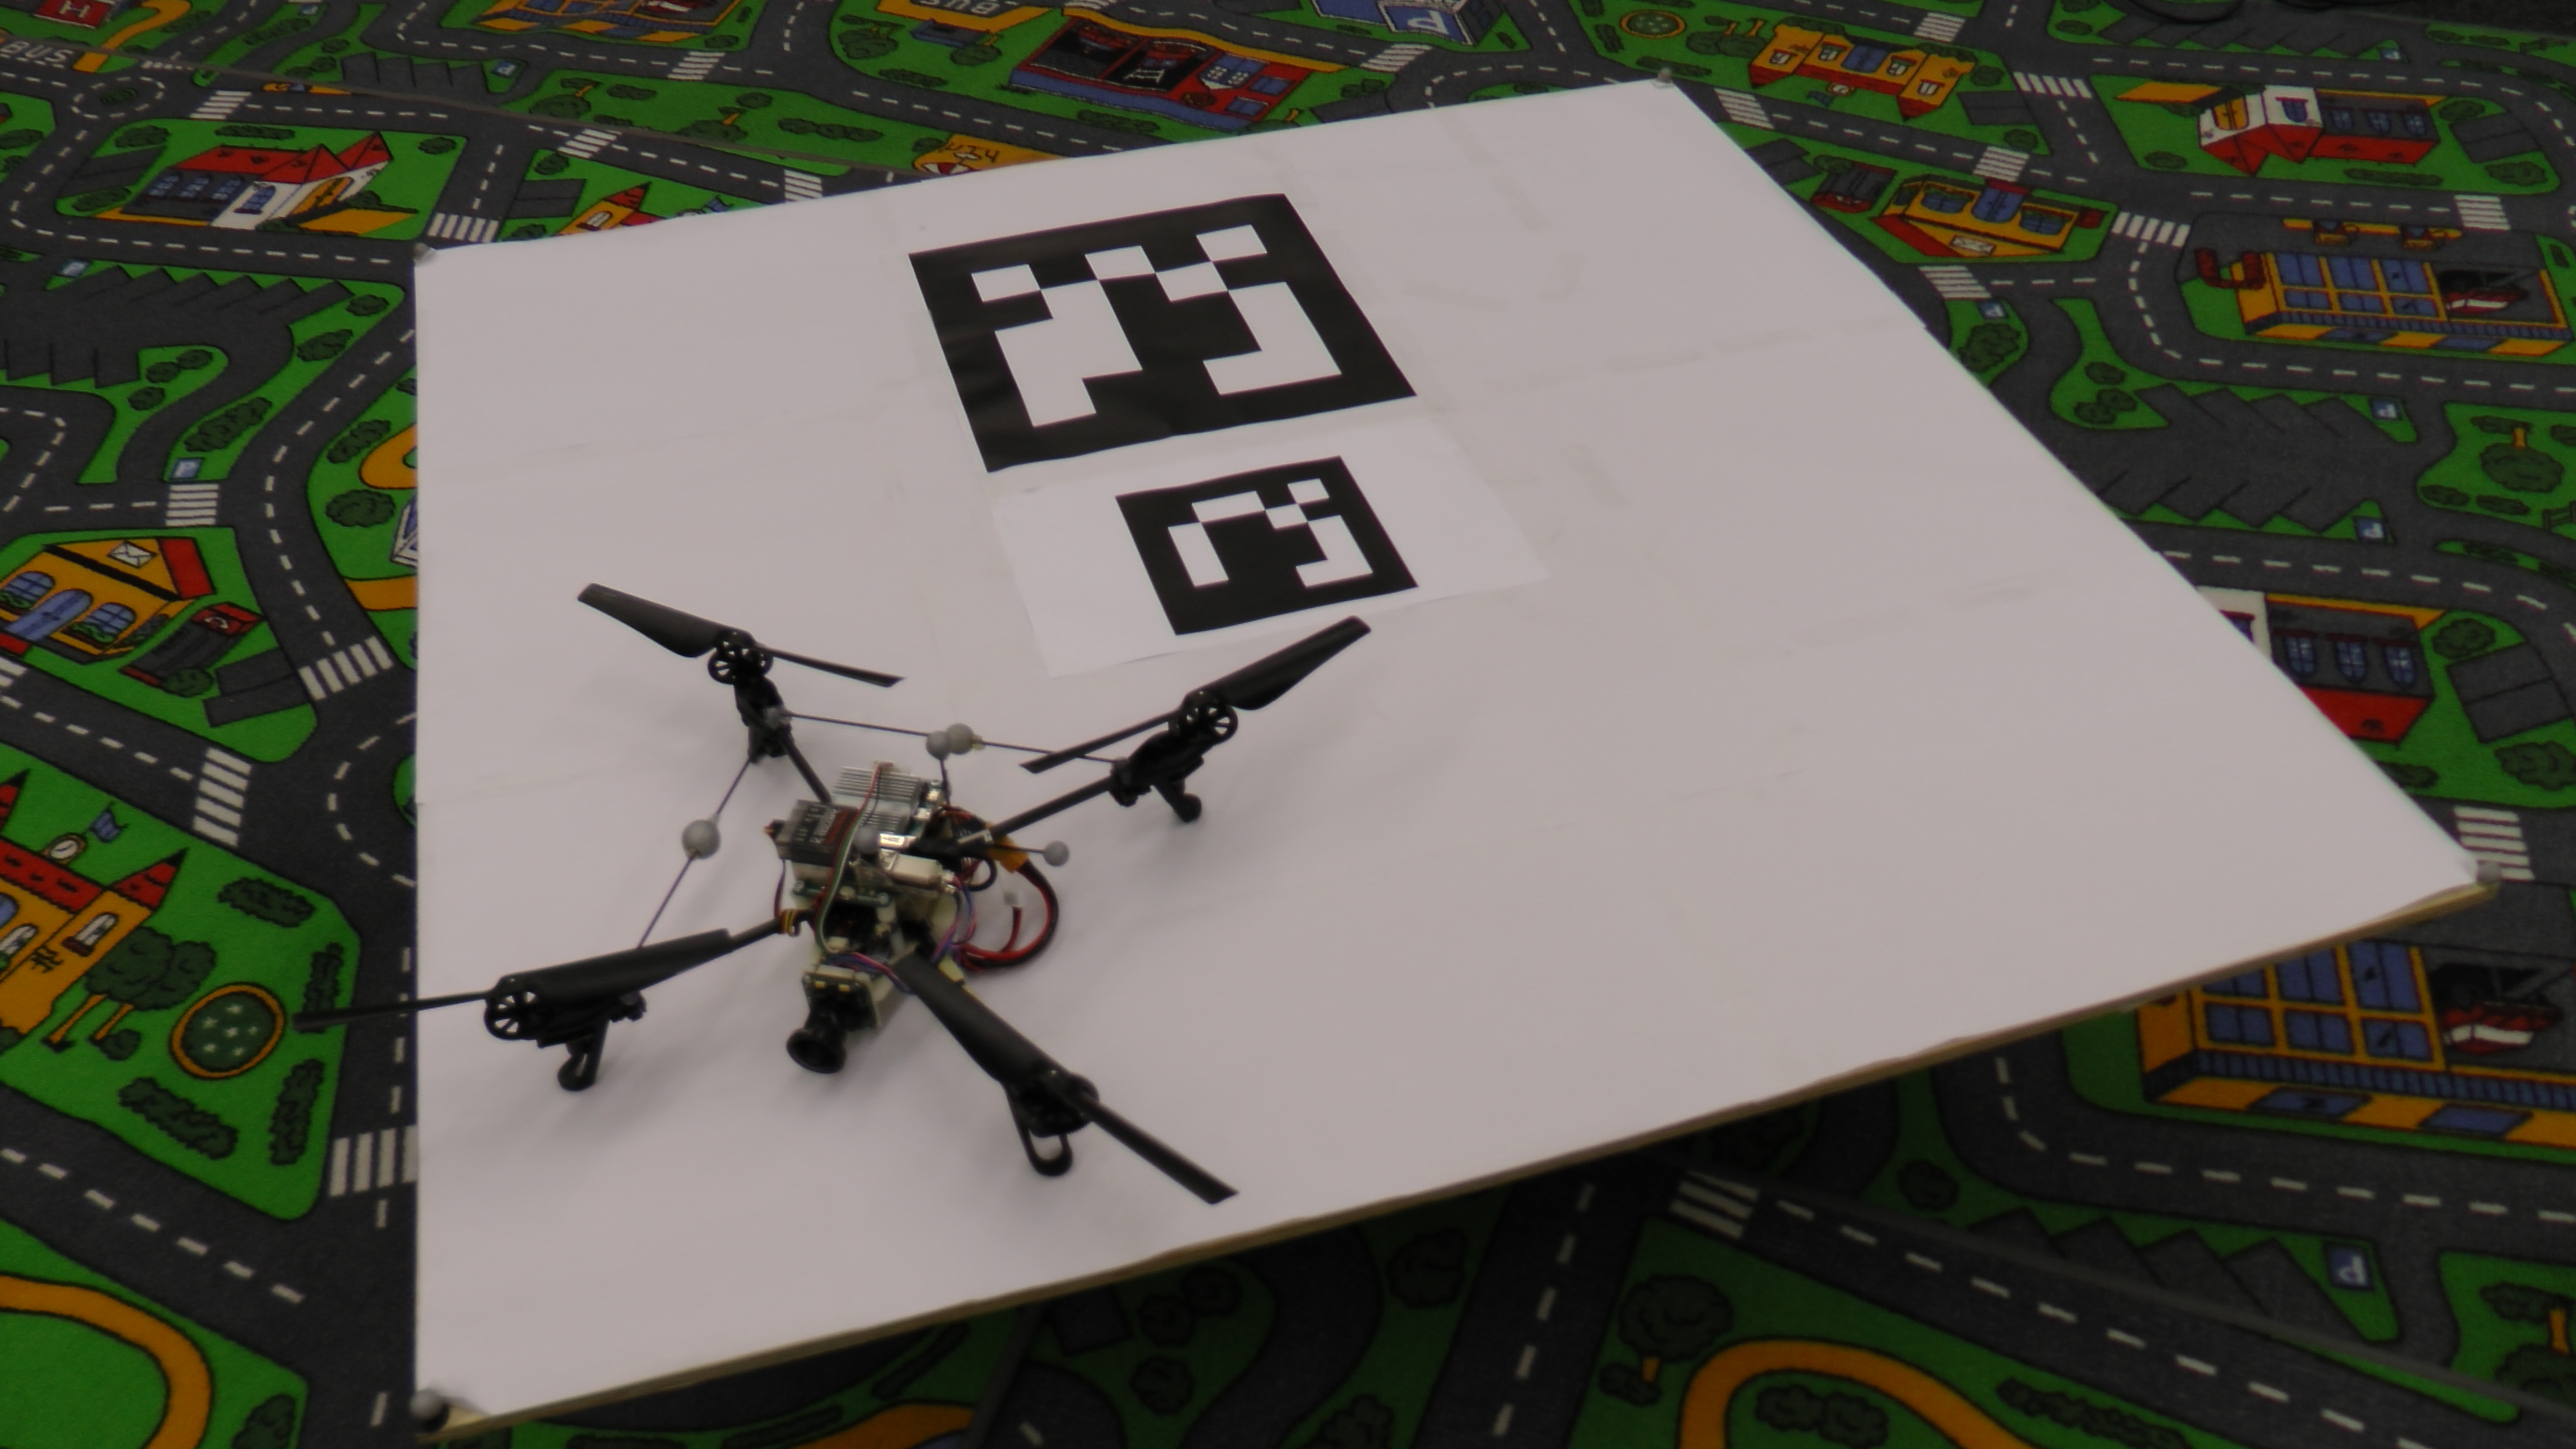
\includegraphics[width=1.0\textwidth]{img/real_world_hardware.jpg}
    \caption{The UAV and UGV used during the experiments}
    \label{fig:quad_hardware}
\end{figure}


\section{Simulation}
A simulation environment is developed in order to recreate as precise as possible the final environment of the challenge.  As a matter of fact, organizing experiments in real field as large as the one in the challenge, can be difficult, but with the simulation environment we can test the whole framework before trying it in the real world.

The simulation is done using Gazebo simulator \cite{gazebosimulator}: it is a free simulation toolbox useful to reproduce populations of robots in complex indoor and outdoor environments, furthermore this toolbox is directly part of ROS.\\
To simulate the quadrotor we use the RotorS simulator \cite{rotors2016}: a UAV Gazebo simulator that provides some multirotor models among which there is the AscTec Hummingbird, very similar to the quadrotor we are using in the real world experiments. All quadrotors can be provided with many sensors such as IMU, cameras etc. \\
To simulate the moving platform we use the ROS package \cite{RobotsHusky} that allows us to control a Clearpath Husky. Over the UGV we installed a platform identical to the one used in the real world.\\

The framework used during the tests in the simulation are the same ones explained in Chap.~\ref{chap:general_framework}, with the difference that the state estimation is not coming from SVO+MSF, but is given by Gazebo and we corrupted it with a Gaussian noise with 0 mean and $\sigma^2$ variance.

\begin{figure}[!ht]
    \centering
    \includegraphics[width=1.0\textwidth]{img/simulation.jpg}
    \caption{The UAV and UGV used during the experiments in simulation}
    \label{fig:quad_ugv_sim}
\end{figure}

\section{SVO}
For this project we need to use a front looking camera for the visual odometry, because, when the UAV is over the base, the majority of the image from the down looking camera is occluded by the platform itself.\\
This is a crucial problem because the features on the base cannot be considered: the perceived movement is relative to the moving platform and not to the world frame. For example, in the scenario in which the quadrotor and the platform are moving with the same velocity, the images taken from the camera are not changing over time, even if the camera is moving. In this case the visual odometry fails to provide reliable results.\\
In the final parts of the mission, using the down looking camera, there will be not enough good features to track  for UAV state estimation, so is necessary to use a front looking camera for self state estimation.

\subsection{Front looking vs down looking}
To compare the results of front looking and down looking SVO we took datasets in which we run two instances of SVO (using the two different images from the two cameras) to compute the pose estimation of the quadrotor and then filter these pose with MSF using the same IMU signal. These state estimations are compared also with the ground truth from the OptiTrack. This way we can compare the two versions of SVO+MSF with the real pose.

The following images show the the results of one of these experiments. In this particular test we hold the quadrotor by hand and we move it inside the flyingroom simulating a square trajectory Fig.~\ref{fig:comparision_svo_trajectory}.

\begin{figure}[!htbp]
    \centering
    \includegraphics[width=0.9\textwidth]{img/comparision_between_two_svo_and_opti_trajectory.pdf}
    \caption{Comparison between SVO position estimation in 3D world. The blue line is the estimation with down looking camera, the red line with front looking one and the black line the ground truth given by the OptiTrack}
    \label{fig:comparision_svo_trajectory}
\end{figure}

In particular, Fig.~\ref{fig:comparision_svo_position} shows the position , Fig.~\ref{fig:comparision_svo_angles} the orientation and Fig.~\ref{fig:comparision_svo_velocities} the velocity estimations from the two versions of SVO compared to the OptiTrack.
 
\begin{figure}[!ht]
    \centering
    \includegraphics[width=0.8\textwidth]{img/comparision_between_two_svo_and_opti_position.pdf}
    \caption{Comparison between SVO position estimations with the front looking camera (dashed lines), down looking camera (solid) and optitrack (black).}
    \label{fig:comparision_svo_position}
\end{figure}

\begin{figure}[!ht]
    \centering
    \includegraphics[width=0.8\textwidth]{img/comparision_between_two_svo_and_opti_angles.pdf}
    \caption{Comparison between SVO orientation estimations with the front looking camera (dashed lines), down looking camera (solid lines) , and OptiTrack (black lines). The orientation data from the OptiTrack are low pass filtered in order to eliminate the high frequency noise.}
    \label{fig:comparision_svo_angles}
\end{figure}

\begin{figure}[!ht]
    \centering
    \includegraphics[width=0.8\textwidth]{img/comparision_between_two_svo_and_opti_velocities.pdf}
    \caption{Comparison between SVO position estimations with the front looking camera (dashed lines), down looking camera (solid lines), and OptiTrack (black lines). The velocity data from the OptiTrack are low pass filtered in order to eliminate the high frequency noise. }
    \label{fig:comparision_svo_velocities}
\end{figure}

We can see that both versions of our estimation framework provide a reliable estimation of the quadrotor pose and velocity. In order to evaluate the precision of the two estimations, see Fig.~\ref{fig:comparision_svo_error}, where the average position error between the two versions of SVO is shown: error generally below \SI{10}{\centi \meter} with RMSE of \SI{4.5}{\centi \meter} for the down looking camera and \SI{6}{\centi \meter} for the front looking one.\\

\begin{figure}[!ht]
    \centering
    \includegraphics[width=0.9\textwidth]{img/comparision_between_two_svo_and_opti_error.pdf}
    \caption{Mean error between the 3D position estimations of the two versions of SVO and the ground truth. Blue line is the error with the down looking camera, the red line with the front looking one. The correspondent dashed lines are the RMSE for the two estimations.}
    \label{fig:comparision_svo_error}
\end{figure}

%This error is larger then expected. In particular the graphs \ref{fig:perc_error} shows the percentage error of the position estimations, related to the maximum distance traveled in each direction. We can see that the error is below $6\%$ in $x,y$ and $8\%$ in $z$ that correspond to a general absolute error smaller than $10cm$.

%\begin{figure}[!htbp]
%  \centering
%  \begin{subfigure}[b]{0.3\textwidth}
%        \includegraphics[width=\textwidth]{img/err_perc_2_svo_x.pdf}
%        \label{fig:perc_errorone}
%   \end{subfigure} \hfill
%   \begin{subfigure}[b]{0.3\textwidth}
%        \includegraphics[width=\textwidth]{img/err_perc_2_svo_y.pdf}
%        \label{fig:perc_errortwo}
%   \end{subfigure}\hfill
%   \begin{subfigure}[b]{0.3\textwidth}
%        \includegraphics[width=\textwidth]{img/err_perc_2_svo_z.pdf}
%        \label{fig:perc_errorthree}
%   \end{subfigure}
%  \caption{Percentage error, in each dimension, between the two version of SVO and the ground truth given by the OptiTrack. The quad traveled more or less 2m in x,y direction and 1m in z.}
%  \label{fig:perc_error}
%\end{figure} 

From Fig.~\ref{fig:comparision_svo_trajectory} we can see that the main problem is the scale factor. The scale factor is estimated at the beginning, tracking features of the images and setting their depth at a known value. If there is an error in this initialization then all the world is scaled and will result bigger or smaller than the reality.


%
%\subsection{Drifting}
%We made other experiments to understand if the current version of frontlooking-fisheye-SVO is good enough to fly with it.\\ 
%We performed several manual flights in the flyingroom, with the same results: generally SVO is estimating a correct and precise state of the quad, but sometimes it occurs that the state estimation drifts.\\
%For example, the dataset shown in Fig.~\ref{fig:svo_position_driftind} is related to a flight in which three times the SVO estimation drifted with respect to the real world in all three axes. We highlighted in the figure these moments.\\
%
%\begin{figure}[!htbp]
%  \centering
%  \begin{subfigure}[b]{0.35\textwidth}
%        \includegraphics[width=\textwidth]{img/fly_with_landing_position.pdf}
%        \label{fig:comparision_svo_position_drifting}
%   \end{subfigure} \hfill
%   \begin{subfigure}[b]{0.3\textwidth}
%        \includegraphics[width=\textwidth]{img/fly_with_landing_trajectory_x.pdf}
%        \label{fig:comparision_svo_position_drifting_x}
%   \end{subfigure}\hfill
%   \begin{subfigure}[b]{0.3\textwidth}
%        \includegraphics[width=\textwidth]{img/fly_with_landing_trajectory_y.pdf}
%        \label{fig:comparision_svo_position_drifting_y}
%   \end{subfigure}
%  \caption{Manual flight in which SVO drifted away from the reality. Highlighted by circles are the moment in which these drifts happened and there are the correspondences between the time domain and the trajectory. }
%  \label{fig:svo_position_driftind}
%\end{figure} 
%
%The reasons for this behavior can be related to the lack of features that the vertical walls in the flyingroom has. As a matter of fact if there are no enough distinctive features the visual odometry can drift. TODO ???

%\subsection{Fast flight}
%In the final challenge the moving car will move at \SI{15}{\km \per \hour} that means \SI{4.17}{\meter \per \second}. In order the quadrotor to be able to follow and land on the platform it must flight faster then this velocity.\\
%With the quadrotor used in this experiments we can reach velocity up to \SI{2}{\meter \per \second}.
%We made some experiments to understand if the state estimation with the front looking camera it is precise at this speed.\\
%The results are reported in Figure \ref{fig:highspeed} that shows a behavior similar


\section{Base detection and tracking}
Several experiments were performed both in simulation and in the real world to evaluate the performance of the platform state estimation.

\subsection{From high altitude}
We do not require the state estimation from high altitude to be very precise, since we need a rough estimation of the position of the platform.
The precision of the estimation depends on the altitude from which the quadrotor is tracking the base and, with the designed EKF, we obtain a reliable estimate of the base state.\\
Figures~\ref{fig:ekf_real_world_high} and \ref{fig:ekf_high_altitude_comparison} show the result of different experiments both in the real world and simulation.\\

In real world experiments we tested the detector with the platform described before. To have a comparison with a ground truth we did the experiments in the RPG flyingroom, where the position of the platform from the OptiTrack is available. In these experiments the quadrotor cannot reach high altitude and it tracks the moving platform from \SI{2}{\meter}.
\begin{figure}[!htbp]
  \centering
   \begin{subfigure}[b]{0.45\textwidth}
        \includegraphics[width=\textwidth]{img/tag_moving_real_world_pos_high_altitude.pdf}
        \caption{Position }
        \label{fig:one_ekf_real_world_high}
   \end{subfigure}\hfill
   \begin{subfigure}[b]{0.45\textwidth}
        \includegraphics[width=\textwidth]{img/tag_moving_real_world_vel_high_altitude.pdf}
        \caption{Velocity}
        \label{fig:two_ekf_real_world_high}
   \end{subfigure}
  \caption{Real world experiment. Comparison between estimate position and velocity with the ground truth values for a  platform moving at \SI{0.2}{\meter \per \second}. The estimate position  is taken from \SI{2}{\meter} height and has a RMSE of \SI{5}{\centi \meter} in $x,y$ and \SI{10}{\centi \meter} in $z$.}
  \label{fig:ekf_real_world_high}
\end{figure} 

In simulation we can track the platform from really high altitude. Figure~\ref{fig:ekf_high_altitude_comparison} shows the result of a tracking from \SI{15}{\meter} height. Of course, in this case the estimate is no long very precise, because the precision of the pose estimation of the platform decreases at high altitude. 

\begin{figure}[!htbp]
  \centering
  \begin{subfigure}[b]{0.5\textwidth}
        \includegraphics[width=\textwidth]{img/high_altitude_error_xy.pdf}
        \caption{Trajectory}
        \label{fig:one}
   \end{subfigure} \\
   \begin{subfigure}[b]{0.35\textwidth}
        \includegraphics[width=\textwidth]{img/high_altitude_error_x.pdf}
        \caption{x }
        \label{fig:one}
   \end{subfigure}
   \begin{subfigure}[b]{0.35\textwidth}
        \includegraphics[width=\textwidth]{img/high_altitude_error_y.pdf}
        \caption{y}
        \label{fig:two}
   \end{subfigure}
  \caption{Comparison between estimate position (blue dots) and real position (green line) in simulation. The platform is moving in the 8 shape path at \SI{1.5}{\meter \per \second} and the quadrotor explores the area at \SI{15}{\meter} of altitude.}
  \label{fig:ekf_high_altitude_comparison}
\end{figure} 

As one can see from Fig.~\ref{fig:ekf_high_altitude_error}, the estimation error can be really high during this phase, as shown by the average error in $x$ and $y$ directions and the correspondent RMSE from a searching at \SI{15}{\meter} of altitude. In general, the state estimate has a RMSE of \SI{0.4}{\meter}.\\
Even if they are not very accurate, this data are good enough to perform the first stages of the state machine.
\begin{figure}[!ht]
    \centering
    \includegraphics[width=0.6\textwidth]{img/high_altitude_error.pdf}
      \caption{Average error between estimate and real x,y coordinate. The RMSE is below \SI{0.4}{\meter}. This precision is sufficient to estimate the type of movement of the base.}
    \label{fig:ekf_high_altitude_error}
\end{figure}


\subsection{From low altitude}
\subsubsection{Different AR-Tag detector}
In the real world implementation we tried several different tag detector ROS packages, such as RPG-April-Tags \cite{rpgapriltags} that uses the AprilTags library \cite{apriltagslibrary}, AR-Sys \cite{arsys} and AR-Track-Alvar \cite{artrackalvar}.\\
All of them have some strengths and weaknesses and we compared the most important features to understand which detector is the more suitable for our purpose:
\begin{itemize}
\item \textbf{Light conditions}: all these methods use the edge based approach, so the results is similar in different light conditions.
\item \textbf{Final pose}: all trackers solve a PnP Problem to find the 6DoF pose of the camera that minimizes the reprojection error of the points in the image. The final result is the transformation between the tag and the camera. RPG-AprilTag has also the possibility to return a 4DoF pose (perfect for our application), saving some computation.
\item \textbf{Multiple tags}: AR-Sys and AR-Track-Alvar have the ability to directly track multiple tags or single target composed by multiple tags.
\item \textbf{Precision}: we measure the error at \SI{1}{\meter} distance from the tag
\begin{itemize}
\item RPG-April-Tags: $\pm$ 1 pixel 
\item AR-Sys: $\pm$ 2 pixel 
\item AR-Track-Alvar: $\pm$ 1 pixel 
\end{itemize}
\item \textbf{Frequency}: on the quadrotor the performance of the three tracker where quite different
\begin{itemize}
\item RPG-April-Tags: $~$\SI{1}{\Hz}
\item AR-Sys: $~$\SI{4}{\Hz}
\item AR-Track-Alvar: $~$\SI{1}{\Hz}
\end{itemize}
\end{itemize}

\paragraph{AR-Sys}
In our final implementation we decided to use AR-Sys because of its computational efficiency. AR-Sys is 3D pose estimation ROS package that uses ARUco marker boards \cite{Aruco2014}.\\
This package guarantees a good error correction in the identification of a specific tag, and, more interesting for our application, a solution to the occlusion problem using multiple markers: it can track the pose of boards composed by multiple tags, considered as a single unit. We can define one of these boards in an XML file. In this file all the tags, that compose the board, are listed. The tags are defined with an ID and with a relative position with respect to a master tag (the first in the list) that defines the center of the cumulative target.
The pose of the camera is given with respect to this master tag. This feature guarantees more stable pose estimates and robustness to the occlusion of a part of the platform.

Very accurate pose estimation is obtain when the AR tags are used. Generally, the error in the $x,y$ coordinate is less then \SI{7}{\centi \meter}, in the $z$ direction is about \SI{3}{\centi \meter}.\\
The following figures show different experiments in the real world and in the simulation with different velocities and initial values.\\

\begin{figure}[!htbp]
  \centering
   \begin{subfigure}[b]{0.45\textwidth}
        \includegraphics[width=\textwidth]{img/tag_static_real_world_pos.pdf}
        \caption{Position }
        \label{fig:one_ekf_real_world_static}
   \end{subfigure}\hfill
   \begin{subfigure}[b]{0.45\textwidth}
        \includegraphics[width=\textwidth]{img/tag_static_real_world_vel.pdf}
        \caption{Velocity}
        \label{fig:two_ekf_real_world_static}
   \end{subfigure}
  \caption{Real world experiment. Comparison between estimate position and velocity with the ground truth values for a static platform. The estimate position has a RMSE of \SI{5}{\centi \meter} in $x,y$ and \SI{2.5}{\centi \meter} in $z$.}
  \label{fig:ekf_real_world_static}
\end{figure} 

\begin{figure}[!htbp]
  \centering
   \begin{subfigure}[b]{0.45\textwidth}
        \includegraphics[width=\textwidth]{img/tag_moving_real_world_pos.pdf}
        \caption{Position }
        \label{fig:one_ekf_real_world_moving}
   \end{subfigure}\hfill
   \begin{subfigure}[b]{0.45\textwidth}
        \includegraphics[width=\textwidth]{img/tag_moving_real_world_vel.pdf}
        \caption{Velocity \SI{0.2}{\meter \per \second}}
        \label{fig:two_ekf_real_world_moving}
   \end{subfigure}
    \centering
   \begin{subfigure}[b]{0.45\textwidth}
        \includegraphics[width=\textwidth]{img/tag_moving_real_world_pos2.pdf}
        \caption{Position}
        \label{fig:one_ekf_real_world_moving2}
   \end{subfigure}\hfill
   \begin{subfigure}[b]{0.45\textwidth}
        \includegraphics[width=\textwidth]{img/tag_moving_real_world_vel2.pdf}
        \caption{Velocity  \SI{1.0}{\meter \per \second}}
        \label{fig:two_ekf_real_world_moving2}
   \end{subfigure}
  \caption{Real world experiment. Comparison between estimate position and velocity with the ground truth values for a platform moving at: figures (a)(b) \SI{0.2}{\meter \per \second}, figure (c)(d) \SI{1.0}{\meter \per \second}. The estimate position has a RMSE of \SI{3}{\centi \meter} in $x,y,z$.}
  \label{fig:ekf_real_world_moving}
\end{figure} 

\begin{figure}[!htbp]
  \centering
   \begin{subfigure}[b]{0.45\textwidth}
        \includegraphics[width=\textwidth]{img/tag_2ms_simulation_pos.pdf}
        \caption{Position }
        \label{fig:one_ekf_simulation_2ms}
   \end{subfigure}\hfill
   \begin{subfigure}[b]{0.45\textwidth}
        \includegraphics[width=\textwidth]{img/tag_2ms_simulation_vel.pdf}
        \caption{Velocity}
        \label{fig:two_ekf_simulation_2ms}
   \end{subfigure}
  \caption{Simulation test. Comparison between estimate position and velocity with the ground truth values. The velocity is initialized with a wrong value of \SI{1}{\meter \per \second} but the filter needs few steps to converge to the right value of \SI{2}{\meter \per \second}. The estimate position has a RMSE of \SI{10}{\centi \meter} in $x,y$ and \SI{2}{\centi \meter} in $z$.}
  \label{fig:ekf_simulation_2ms}
\end{figure} 


%\begin{figure}[!htbp]
%  \centering
%   \begin{subfigure}[b]{0.45\textwidth}
%        \includegraphics[width=\textwidth]{img/tag_2ms_simulation_pos.pdf}
%        \caption{Position }
%        \label{fig:one}
%   \end{subfigure}\hfill
%   \begin{subfigure}[b]{0.45\textwidth}
%        \includegraphics[width=\textwidth]{img/tag_2ms_simulation_vel.pdf}
%        \caption{Velocity}
%        \label{fig:two}
%   \end{subfigure}
%  \caption{Simulation test. Comparison between estimate position and velocity with the ground truth values. The velocity is initialized with 0 value. In this case the filter needs some time to converge to the right value of velocity.}
%  \label{fig:ekf_simulation_hot_init}
%\end{figure}


\section{Trajectory generation}

\subsection{Acceleration estimation} \label{subsec:acceleration_experiments}
We described in Sec.~\ref{subsec:acceleration} the three possible methods to estimate the acceleration of the quadrotor at a given time. This calculation is necessary because the trajectory generator needs a full state description of the initial condition of the quadrotor [position,velocity,acceleration] in order to solve the optimal control problem.\\
We took several datasets while the quadrotor was flying in the flyingroom in order to compare the different methods used to estimate the accelerations.\\

Figure~\ref{fig:comparison_acc} compares the accelerations estimated with IMU measurements, with finite difference calculated with two subsequent velocity estimations, and with the total thrust. On the left column we considered the raw data, while on the right column we consider the filtered versions of the accelerations calculated with finite difference and with the data from the IMU.
\begin{figure}[!htbp]
 \centering   
     \begin{subfigure}[b]{0.45\textwidth}
     \includegraphics[width=\textwidth]{img/acceleration_mass_changed_no_filter_x.pdf}
        \caption{Acceleration x axis not filtered}
        \label{fig:comparison_accx}
   \end{subfigure}
    \begin{subfigure}[b]{0.45\textwidth}
     \includegraphics[width=\textwidth]{img/acceleration_mass_changed_filtered_x.pdf}
        \caption{Acceleration x axis filtered}
        \label{fig:comparison_accx_fil}
   \end{subfigure}\\[20pt]
   
   \begin{subfigure}[b]{0.45\textwidth}
     \includegraphics[width=\textwidth]{img/acceleration_mass_changed_no_filter_y.pdf}
        \caption{Acceleration y axis  not filtered}
        \label{fig:comparison_accy}
   \end{subfigure}
    \begin{subfigure}[b]{0.45\textwidth}
     \includegraphics[width=\textwidth]{img/acceleration_mass_changed_filtered_y.pdf}
        \caption{Acceleration y axis filtered}
        \label{fig:comparison_accy_fil}
   \end{subfigure}\\[20pt]
   
    \begin{subfigure}[b]{0.45\textwidth}
     \includegraphics[width=\textwidth]{img/acceleration_mass_changed_no_filter_z.pdf}
        \caption{Acceleration z axis  not filtered}
        \label{fig:comparison_accz}
   \end{subfigure}
     \begin{subfigure}[b]{0.45\textwidth}
     \includegraphics[width=\textwidth]{img/acceleration_mass_changed_filtered_z.pdf}
        \caption{Acceleration z axis filtered}
        \label{fig:comparison_accz_fil}
   \end{subfigure}
    \caption{Comparison between the accelerations calculate with the three different methods. On the left side the raw data without filtering IMU and finite difference measurements. On the right column the same dataset, but with filtered version for IMU and finite difference.}
    \label{fig:comparison_acc}
\end{figure}

It is easy to notice that only the raw data from the thrust can be considered a good approximation of the acceleration, while the other two signals need some filtering. On the other hand, the filtered version of IMU and finite differences, are smooth but they have some delays.\\

Figure~\ref{fig:comparison_acc} shows that there is some offset between the three different approximations: in particular, in the z direction this difference between the acceleration computed with the thrust and the other two methods is very clear.\\
This offset is more evident in the Fig.~\ref{fig:comparison_acc_mass} where the right graph is the same Fig.~\ref{fig:comparison_accz_fil}, while the left part is calculate with the same data set, but the mass of the quadrotor is modify by the $5\%$ from \SI{515}{\gram} to \SI{545}{\gram}. This tiny modification is creating a big difference in the final acceleration.

\begin{figure}[!htbp]
 \centering   
  \begin{subfigure}[b]{0.45\textwidth}
     \includegraphics[width=\textwidth]{img/acceleration_mass_correct_filtered_z.pdf}
        \caption{Acceleration z axis filtered with real mass of 545g}
        \label{fig:comparison_accz_mass}
   \end{subfigure}
     \begin{subfigure}[b]{0.45\textwidth}
     \includegraphics[width=\textwidth]{img/acceleration_mass_changed_filtered_z.pdf}
        \caption{Acceleration z axis filtered with modify mass of 515g}
        \label{fig:comparison_accz_fil_mass}
   \end{subfigure}
    \caption{Comparison between the accelerations calculate with the three different methods. On the left side accelerations calculate considering the real mass of 545g , on the right column considering 545g}
    \label{fig:comparison_acc_mass}
\end{figure}

Also in the other axis, if we change the mass, we can see that the acceleration estimation computed with the thrust shows an offset with respect to the other two signals.\\ This could be caused by a not precise estimation of the rotor fitness factors.\\

\section{Landing on a moving platform}
We also made different trials of the entire framework, in order to understand if all the pieces linked together are good enough to complete the task.\\
In simulation we reached velocity of the moving platform of up to \SI{3}{\meter \per \second}, while in the real world we managed to achieve velocity of \SI{0.6}{\meter \per \second} for the platform. \\
We achieved a successful landing rate of over $90\%$.\\
The main issues why we have not tried yet higher velocity in the real world is that the quadrotor we are using has hardware limitations that do not allow fast trajectory tracking, so in the final stages of the state machine, the trajectory generator is not able to find feasible trajectories that bring the quadrotor on the platform. Furthermore, the trajectory replanning at high velocities causes some fast oscillations to the quadrotor, and this may result the failure of the visual odometry. 

Figs. \ref{fig:landing1},  \ref{fig:landing2} and  \ref{fig:landing3}  show pictures from different tests in the real world and in simulation. In each set of pictures we highlighted the stages of the landing state machine. The quadrotor proceeds from a stage to another until it completes the mission and lands on the moving platform.

\begin{figure}[!htbp]
  \centering
   \begin{subfigure}[b]{0.45\textwidth}
        \includegraphics[width=\textwidth]{img/takeoff3.jpg}
        \caption{Takeoff.}
   \end{subfigure}\hfill
   \begin{subfigure}[b]{0.45\textwidth}
        \includegraphics[width=\textwidth]{img/exploring3.jpg}
        \caption{Exploration.}
        \label{fig:two}
   \end{subfigure}\hfill
    \begin{subfigure}[b]{0.45\textwidth}
        \includegraphics[width=\textwidth]{img/following3.jpg}
        \caption{Following the base.}
        \label{fig:three}
   \end{subfigure}\hfill
    \begin{subfigure}[b]{0.45\textwidth}
        \includegraphics[width=\textwidth]{img/approaching3.jpg}
        \caption{Approaching the base.}
        \label{fig:three}
   \end{subfigure}\hfill
   \begin{subfigure}[b]{0.45\textwidth}
        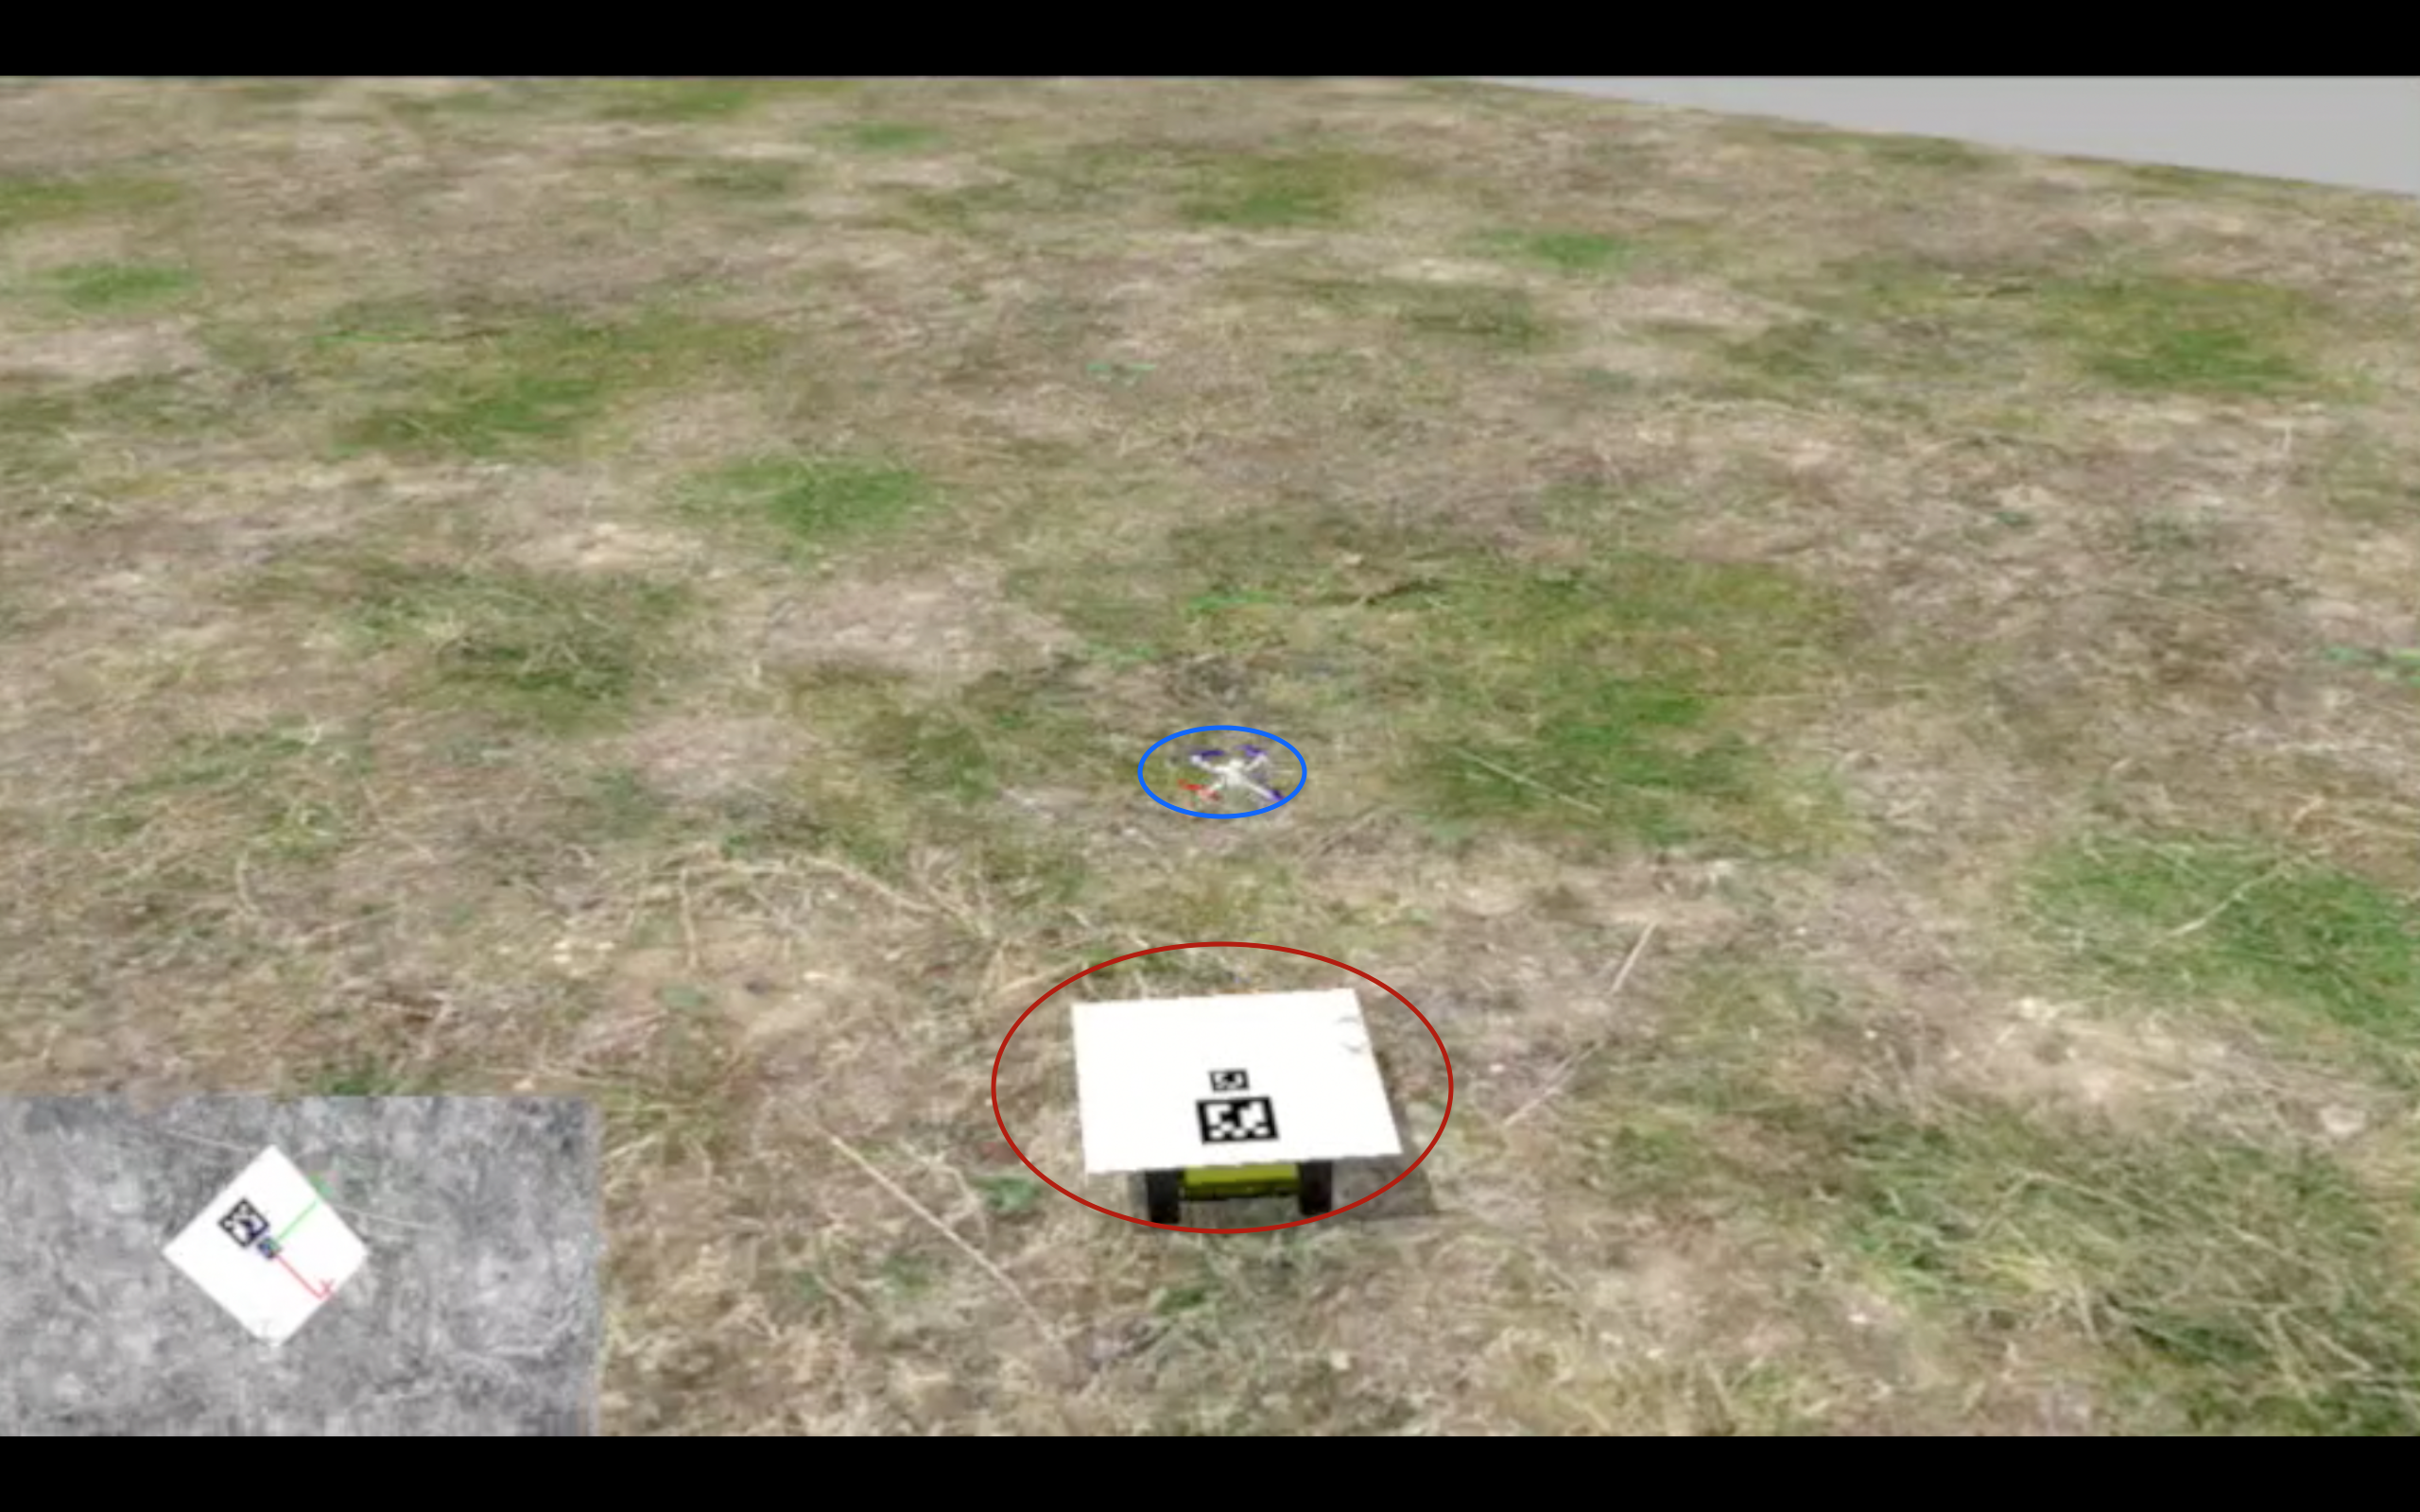
\includegraphics[width=\textwidth]{img/align3.jpg}
        \caption{Align with the base.}
        \label{fig:three}
   \end{subfigure}\hfill
    \begin{subfigure}[b]{0.45\textwidth}
        \includegraphics[width=\textwidth]{img/landing3.jpg}
        \caption{Landing on the base.}
        \label{fig:four}
   \end{subfigure} \hfill
    \begin{subfigure}[b]{0.45\textwidth}
        \includegraphics[width=\textwidth]{img/landed3.jpg}
        \caption{Landed on the base.}
        \label{fig:five}
   \end{subfigure}
   
  \caption{Sequence of images taken from a simulation experiment in which the platform is moving at \SI{2.0}{\meter \per \second} }
  \label{fig:landing1}
\end{figure}

\begin{figure}[!htbp]
  \centering
   \begin{subfigure}[b]{0.5\textwidth}
        \includegraphics[width=\textwidth]{img/takeoff2.jpg}
        \caption{Takeoff.}
   \end{subfigure}
   \begin{subfigure}[b]{0.5\textwidth}
        \includegraphics[width=\textwidth]{img/exploring2.jpg}
        \caption{Exploration.}
        \label{fig:two}
   \end{subfigure}
   \begin{subfigure}[b]{0.5\textwidth}
        \includegraphics[width=\textwidth]{img/align2.jpg}
        \caption{Align with the base.}
        \label{fig:three}
   \end{subfigure}
    \begin{subfigure}[b]{0.5\textwidth}
        \includegraphics[width=\textwidth]{img/landing2.jpg}
        \caption{Landing on the base.}
        \label{fig:four}
   \end{subfigure} 
    \begin{subfigure}[b]{0.5\textwidth}
        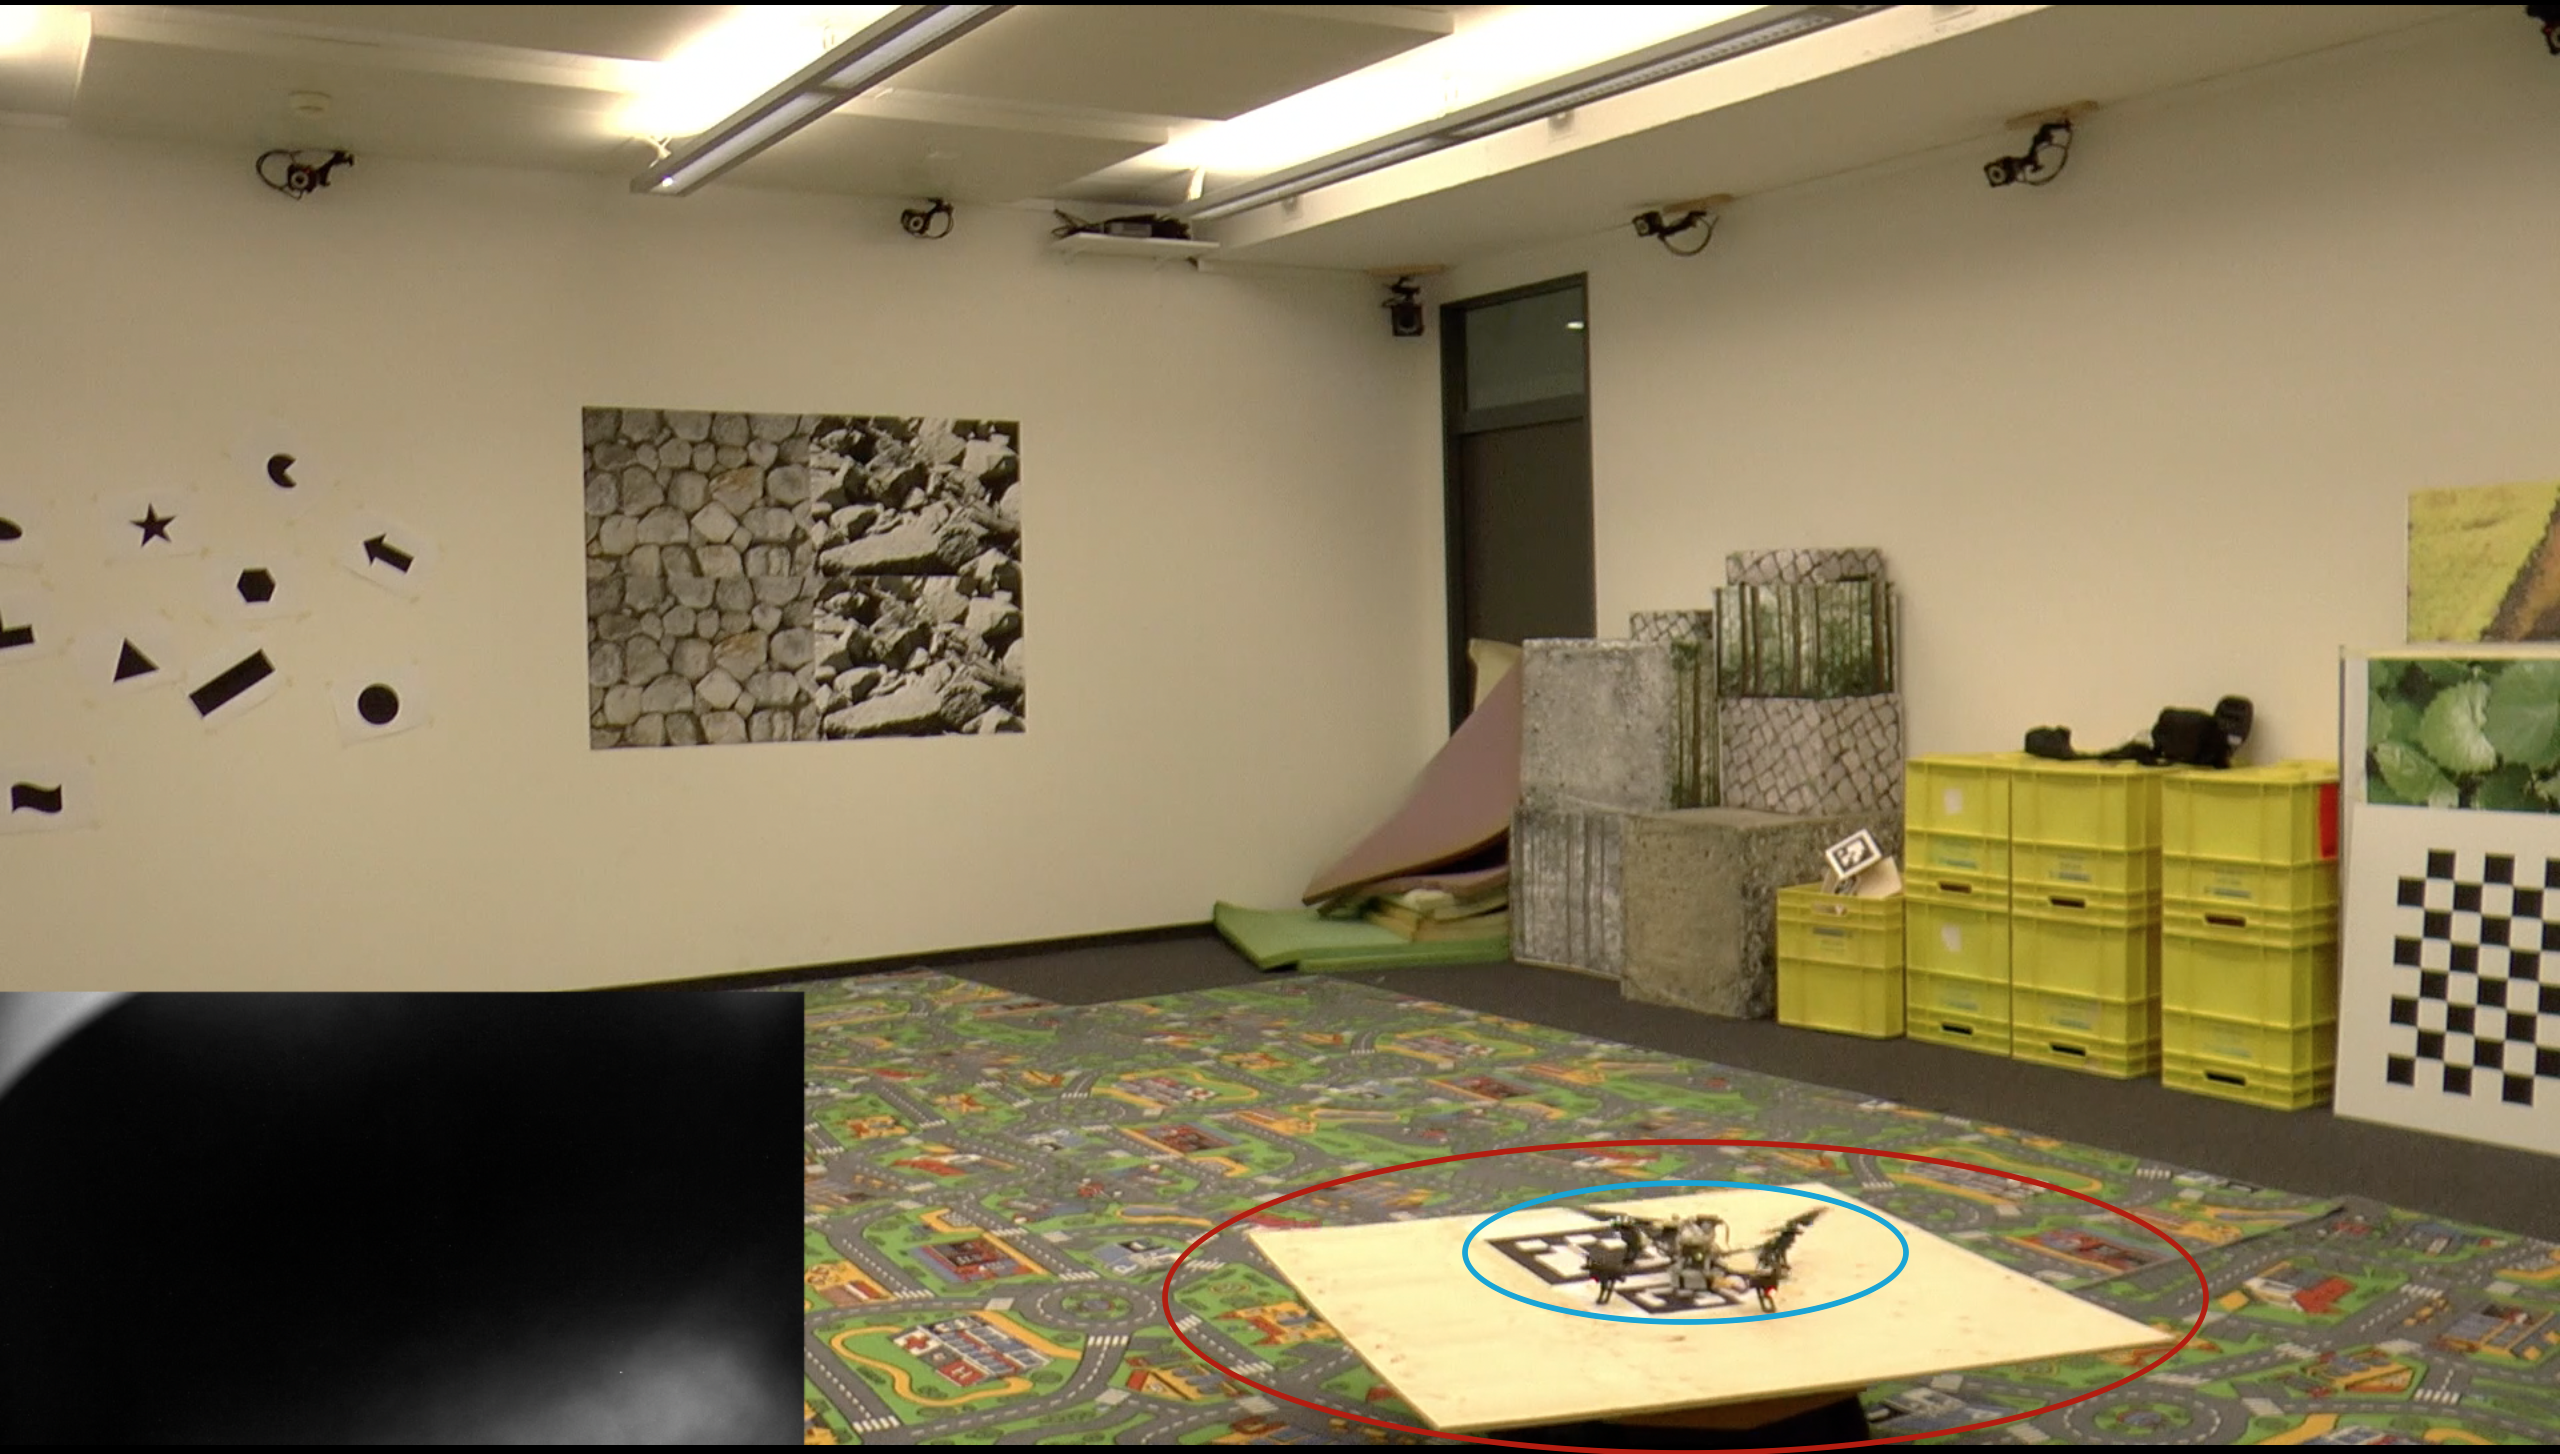
\includegraphics[width=\textwidth]{img/landed2.jpg}
        \caption{Landed on the base.}
        \label{fig:five}
   \end{subfigure}
   
  \caption{Sequence of images taken from a real world experiment in which the platform is moving at \SI{0.5}{\meter \per \second} }
  \label{fig:landing2}
\end{figure} 

\begin{figure}[!htbp]
  \centering
   \begin{subfigure}[b]{0.5\textwidth}
        \includegraphics[width=\textwidth]{img/takeoff1.jpg}
        \caption{Takeoff.}
   \end{subfigure}
   \begin{subfigure}[b]{0.5\textwidth}
        \includegraphics[width=\textwidth]{img/exploring1.jpg}
        \caption{Exploration.}
        \label{fig:two}
   \end{subfigure}
   \begin{subfigure}[b]{0.5\textwidth}
        \includegraphics[width=\textwidth]{img/align1.jpg}
        \caption{Align with the base.}
        \label{fig:three}
   \end{subfigure}
    \begin{subfigure}[b]{0.5\textwidth}
        \includegraphics[width=\textwidth]{img/landing1.jpg}
        \caption{Landing on the base.}
        \label{fig:four}
   \end{subfigure} 
    \begin{subfigure}[b]{0.5\textwidth}
        \includegraphics[width=\textwidth]{img/landed1.jpg}
        \caption{Landed on the base.}
        \label{fig:five}
   \end{subfigure}
   
  \caption{Sequence of images taken from a real world experiment in which the platform is moving at \SI{0.6}{\meter \per \second} }
  \label{fig:landing3}
\end{figure} 




 

%\begin{figure}[h]
%   \centering
%   \includegraphics[width=0.75\textwidth]{img/processing_time.pdf}
%   \caption{Example of a figure.}
%   \label{img:timing}
%\end{figure}